%
% Another appendix chapter
\chapter{Towards Application}
As the control strategy of Chapter \ref{chap:mpc} is in \ac{2D}, in this chapter a new strategy is proposed that is implementable on a real robot. First a experimental setup is shown with preliminary observations, to support assumptions made in the method developped. In the end, results are shown in simulation and on hardware.
% Experimental Setup
\section{Experimental Setup}
Evalutation of the strategy will be done based on push recovery on flat terrain. The situations considered when the push is applied are to be distinguished in two cathegories:
\begin{itemize}
	\item A static case, where the robot is standing
	\item A dynamic case, where the robot is walking
\end{itemize}
In both cathegories, limited foothold options are provided, such that step location adjustment would not be possible. Also, step timing is assumed to be given beforehand and is fixed, to make comparison with other control strategies more straight forward. The control strategies compared with are:
\begin{itemize}
	\item ``Ankle'' strategies: the desired \ac{CMP} is constrained to be inside the support polygon. 
	\item ``Ankle'' and ``Hip'' strategies : the desired \ac{CMP} can leave the support polygon uptil a maximum allowed distance.
\end{itemize}
The stepping parameters used for the walking test situation are given in Table \ref{tab:stepping}.
\begin{table}[ht]
\caption{Stepping Parameters} % title of Table
\centering % used for centering table
\begin{tabular}{c c c } % centered columns (4 columns)
\hline\hline %inserts double horizontal lines
Parameter & Value & Unit \\
%heading
\hline % inserts single horizontal line
Step Legth & 0.5 &  [m]\\
Step Width & 0.25 & [m]\\
\acs{SS} Time & 0.6 & [s]\\
\acs{DS} Time & 0.15 & [s]\\
%[1ex] % [1ex] adds vertical space
\hline %inserts single line
\end{tabular}
\label{tab:stepping} % is used to refer this table in the text
\end{table}
%Preliminary observations
\subsection{Preliminary Observations}
Before developping of a control method, the behavior of the system is studied, to get more insight in its behavior under handling errors. The following properties are observed after applying pushes on the robot from different directions in the experimental setups considered:
\begin{itemize}
	\item Applying a lower weight in the whole-body \ac{QP} on vertical linear momentum rate, causes the robot to use height variation in recovery.
	\item After a push in the swing phase, the direction of the \ac{ICP} error stays approximately the same until transition to \ac{DS}.
	\item If the \ac{ICP} error is directed in the sagittal plane, the desired \ac{CMP} often remains somewhat in the same location.
	\item if the \ac{ICP} error is directed  in the coronal plane, the desired \ac{CMP} slides from back to the forth of the foot.
	\item The configuration and velocity near transition to \ac{DS} affects the robots ability to put its swing leg down at the desired time. Also, the swing leg can collapse at touch down if the negative height velocity is too high.
	\item When the $\dotldz$ is high near the end of \ac{DS}, the robot can have problems with the transition to \ac{SS}.
\end{itemize}
\begin{table}[ht]
\caption{Major affected tasks by $\mathbf{\dot{l}}_{xy,d}$ in whole-body QP, if \ac{CoP} is saturated.} % title of Table
\centering % used for centering table
\begin{tabular}{c c c } % centered columns (4 columns)
\hline\hline %inserts double horizontal lines
Affected Desired & Constraint/Consideration & Centroidal Momentum Rate \\
%heading
\hline % inserts single horizontal line
 $z_d$ & Leg singularity & Linear\\
 $\boldsymbol{\phi}_{body,d}$ & Upper body pose & Angular\\
 $\mathbf{r}_{foot,d}$ &  Touchdown time & Angular\\
%[1ex] % [1ex] adds vertical space
\hline %inserts single line
\end{tabular}
\label{tab:eatqp} % is used to refer this table in the text
\end{table}
\begin{figure}[h]
\centering
  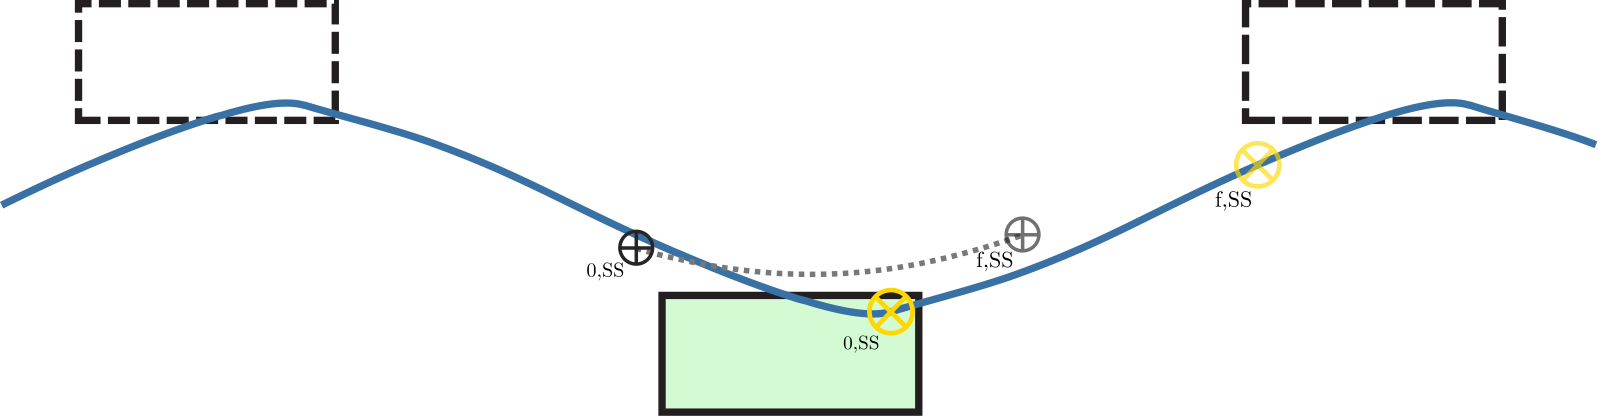
\includegraphics[width=.8\linewidth]{STYLESTUFF/ICPplan3StepComICPrSS.png}
   \caption{Initial (0,SS) and final (f,SS) configurations of \ac{CoM} position (black circle with cross) and \ac{ICP} reference (yellow circle with rotated cross) for \ac{SS} in the $xy$-plane with the parameters from Table \tabref{tab:stepping}. The green area is the current supporting foothold and the blue line is the \ac{ICP} reference trajectory.}
    \label{fig:3foot}
\end{figure}

\newpage
% Methods
\section{Methods}
Other publications that consider \ac{CoM} height variations for balance use \ac{MPC}. Considering worst-case scenario's, where additional horizontal force is needed, `the best you can do' is needed to not fall over. This motivates to use a proportional controller in worst case scenario's, next to the benefit of simplicity and robustness.

%Challenges
\subsection{Motivation}
The controller that uses \ac{CoM} height variations for balance is developped under the motivation that the robot should do the best it can to not fall over. Height variation has the most effect on the horizontal momentum if the robot is relatively far from the point foot \todo{ref section}. Therefore, situations where the controller is allowed to work considers only the scenario's where the \ac{CoP} is saturated.
\paraskip
To make a good comparison with other strategies possible, the controller is designed with the objective to not request additional angular momentum from the robot. Other considerations are kinematic reachability, control in \ac{3D} and the predictability of the dynamics of the system.

%Architecture
\subsection{Control Framework}
To actively change $\dotldxy$, the objective is to generate as few resulting additional angular momentum as possible, compared to the normal control setup. Note that the normal control setup relies on a computed $\rcmpd$ based on the linear model with constant height, as in Equation \eqref{eq:rcmpd} and \eqref{eq:dotldxy}. In the case of the assumption of a \ac{LIP}, the expected angular momentum generated by the robot is a linear function depending on the difference between the \ac{CMP} and \ac{CoP}. If height changes are considered however, having the \ac{CMP} in the same location in one configuration, can request different angular momenta with changing $\fgrz$. The generic formula to write resulting horizontal ground reaction force as a function of the \ac{CMP}  location is:
\begin{equation}
\fgrxy=\frac{\mathbf{c}_{xy}-\mathbf{r}_{cmp}}{z}\fgrz
\label{eq:fgrxygeneric}
\end{equation}
If $\fgrz$ varies and $\rcmp$ remains constant, $\taucom$ has to scale linearly with $\fgrz$, because $\rcmp = \rcop + \frac{\taucom}{\fgrz}$. Therefore, additional horizontal linear momentum rate is requested based on the \ac{CoP}, rather than the \ac{CMP}.
\paragraph{Generation of $\dotldxy$} is done by modifying the desired linear momentum rate from the \ac{LIP}-based PD-controlled setup. Equation \eqref{eq:fgrxygeneric} is rewritten in terms of $\rcop$ in the following way:
\begin{align}
\fgrxy&=\frac{\mathbf{c}_{xy}-(\mathbf{r}_{cop}+\frac{\taucom}{F_z})}{z}\fgrz \\
&=\frac{\mathbf{c}_{xy}-\mathbf{r}_{cop}}{z}m(g+\ddot{z}) - \frac{\taucom}{z} \\
&=\frac{\mathbf{c}_{xy}-\mathbf{r}_{cop}}{z}mg - \frac{\taucom}{z} + \frac{\mathbf{c}_{xy}-\mathbf{r}_{cop}}{z}m\ddot{z}.
\end{align}
Note that for a \ac{LIP} model the following equality holds:
\begin{equation}
	\frac{\mathbf{c}_{xy}-\mathbf{r}_{cop}}{z_0}mg - \frac{\taucom}{z_0} = \frac{\mathbf{c}_{xy}-\mathbf{r}_{cmp}}{z_0}mg.
\end{equation}
For this reason the desired linear momentum rate is modified in the following way:
 \begin{equation}
\dot{\mathbf{l}}_{xy,d}=\underbrace{ \frac{\mathbf{c}_{xy}-\mathbf{r}_{cmp,d}} {z_0}mg}_{\dotldxylip}  + \underbrace{\frac{\mathbf{c}_{xy}-\mathbf{r}_{cop,d}}{z}m\ddot{z}_d}_{\dotldxyheight},
\end{equation}
where $\dotldxylip$ is the already existing desired horizontal linear momentum rate of change from the \ac{ICP} controller and $\dotldxyheight$ is the additional desired momentum rate from height control. The desired \ac{CoP} $\rcopd$ is equal to $\rcmpd$ if $\rcmpd$ is inside the convex support polygon. If $\rcmpd$ is outside the polygon, $\rcopd$ is the orthogonal projection of $\rcmpd$ onto the polygon, as the \ac{CoP} lives by definition inside the support polygon. The desired height acceleration $\ddzd$ is the output of the height controller, which will be discussed in Section \ref{sec:strategy}.
\paragraph{The condition to activate the controller} is when the \ac{ICP} error $\icpe$ is of such length, that \ac{CoP} strategies are no longer sufficient for balance control and an additional input has to be generated. The condition is $\icpe>\fracicp$, where the parameter $\fracicp=0.04$ is found to be a good estimate of the moment when the \ac{CoP} hits the edge of the polygon, considering the control settings at the time of writing \todo{ref to settings}. Also, the controller is only allowed to work in a static case or during the swing phase.

%Strategy 
\subsection{Control Strategy}\label{sec:strategy}


%
\paragraph{Alignment} of the line between $\rcopd$ and $\cxy$ with the vector $\icpe$ is used as a decision variable. If the vectors are perfectly aligned, $\ddzd$ will request $\dotldxyheight$ in the same direction as $\icpe$. This is, considering alignment, the perfect case to use height control. If the vectors are orthogonal, the requested $\dotldxyheight$ will be orthogonal to $\icpe$ and will not help driving back the error. Furthermore, the error in will grow in its orthogonal direction. Height control for any alignment in between the two cases mentioned will have a combined effect in resolving $\icpe$ in its direction, and generating additional error orthogonal to it.

\paragraph{Distance}


\paragraph{Constraints} that are considered are a minimum and maximum height and height velocity. The maximum length of the leg describes a part of a circle throught the swing phase. In the controller, this constraint is captured in two constraints: $\zmaxfirst$, in the first halve of the swing phase and $\zmaxscnd$, in the second part of the swing phase. In \figref{fig:heightconstraints} the two constraints are vizualized. 
\begin{figure}[h]
\centering
  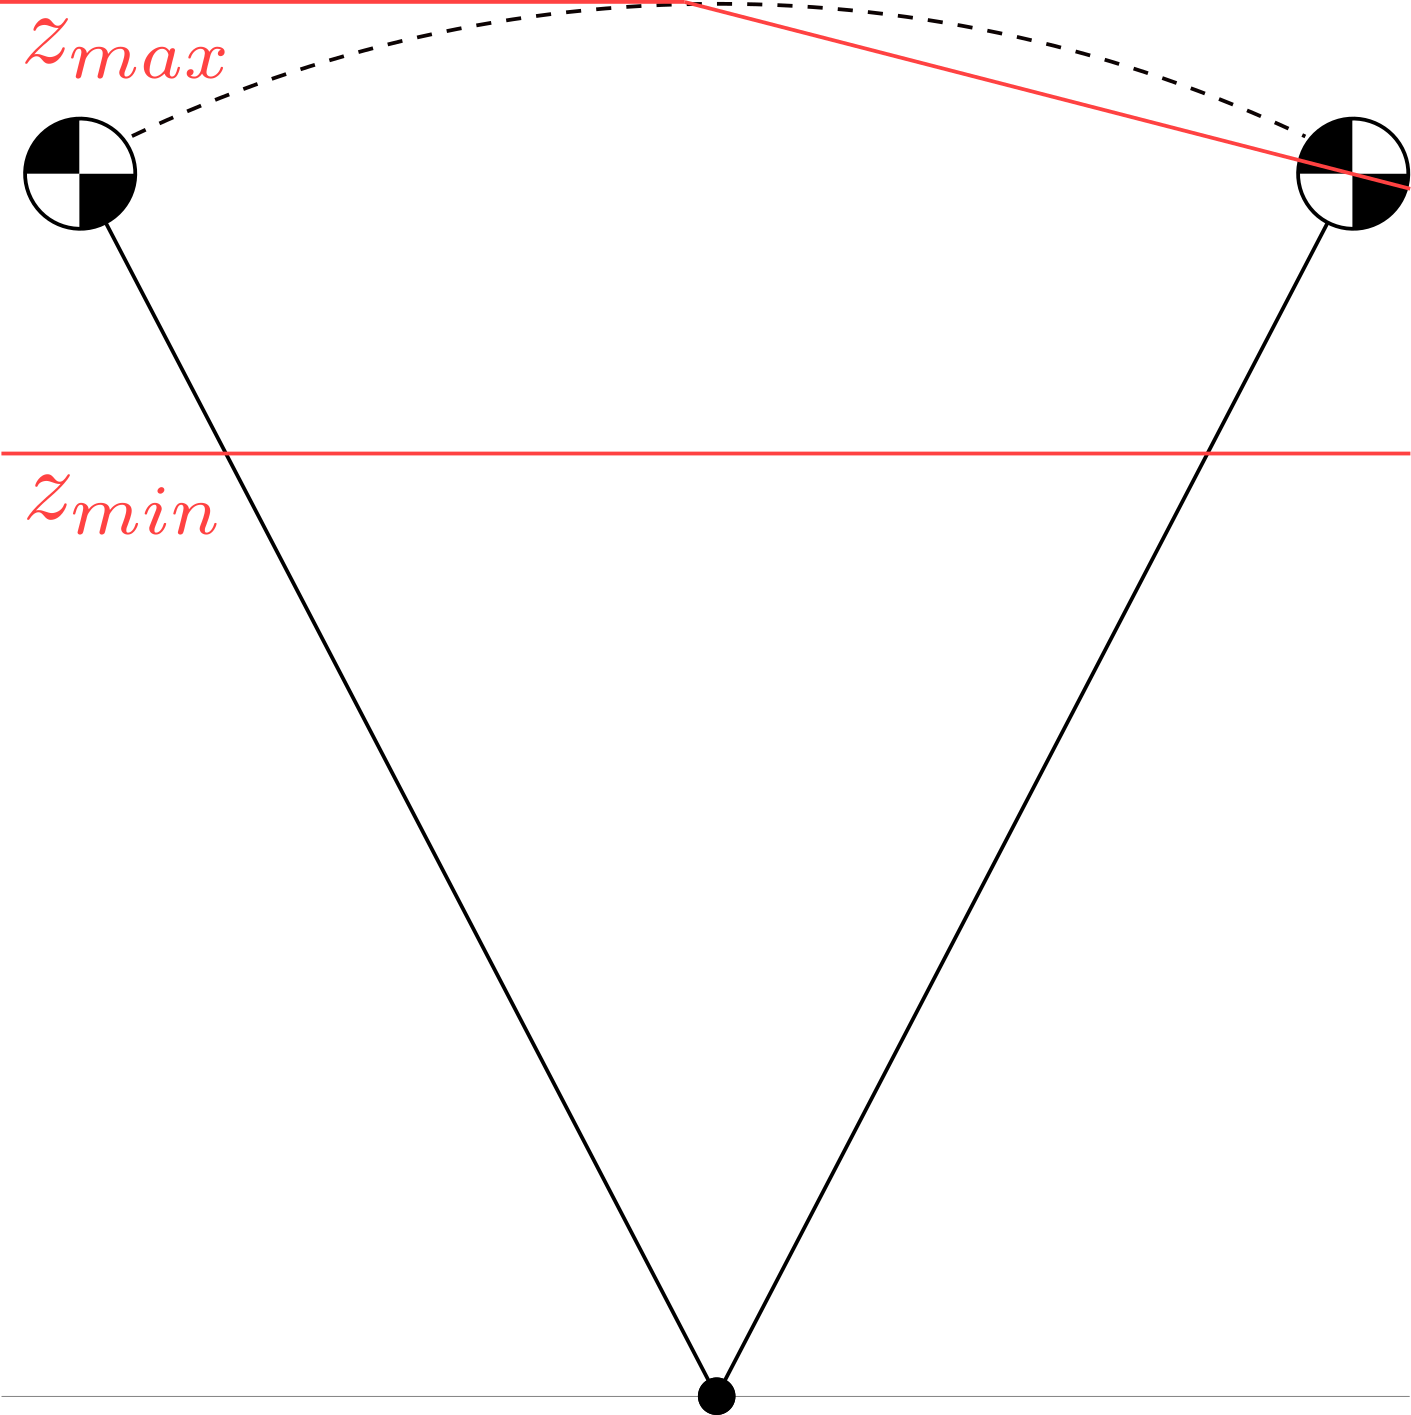
\includegraphics[width=.4\linewidth]{STYLESTUFF/heightconstraints.png}
   \caption{Height constraints through \ac{SS}}
    \label{fig:heightconstraints}
\end{figure} 
The predicted height the current state is about to reach is computed as:
\begin{equation}
	\zmaxpred = z + \sgn(\dot{z})\frac{\dot{z}^2}{-2\ddzminpred},
\end{equation}
where $\zmaxpred$ is the predicted maximum height from the current state and $\ddzminpred$ is the predicted maximum deceleration that will occur. This would be the gravity acceleration, but the minimal acceleration is limited. 
\paraskip
The minimum height constraint is not dependent on singularity of the swing leg and is kept at a constant value. Next to hitting the ground, a low height can cause problems at transfer to \ac{DS}, when the robot gets raised to default height again. The minimum height constraint $\zmin$ is displayed in \figref{fig:heightconstraints}. In a similar way as $\zmaxpred$, the minimum height constraint is computed as:
\begin{equation}
	\zminpred = z - \sgn(\dot{z})\frac{\dot{z}^2}{2\ddzmaxpred},
\end{equation}
where $\zminpred$ is the predicted minimum height from the current state and $\ddzmaxpred$ is the predicted maximum acceleration that will occur.
\paraskip
Contraints on the maximum height velocity $\dzmax$ and minimum height velocity $\dzmin$ are also taken into account. Reasons for this include collapsing of the swing leg at touch down and limited velocities at the robot. 


\subsubsection{Time Prediction To Constraints}
Time to maximum constraint, considered the minimum and maximum acceleration:
\begin{equation}
    z + \dot{z}\tzmax + \frac{1}{2}\ddzdmax\tzmax^2 + \frac{1}{2}\frac{(\dot{z} +\ddzdmax\tzmax)^2}{-\ddzminpred}= \zmax,
\end{equation}
where $\tzmax$ can be computed in the following way:
\begin{equation}
    \underbrace{\frac{1}{2}(\ddzdmax + \frac{\ddzdmax^2}{-\ddzminpred})}_a\tzmax^2 + \underbrace{(\dot{z} + \dot{z}\frac{\ddzdmax}{-\ddzminpred})}_b\tzmax + \underbrace{z - \zmax + \frac{1}{2}\frac{\dot{z}^2}{-\ddzminpred}}_c.
\end{equation}
Noting that $a$ is positive and that the time needs to be the positive solution, the predicted time to the maximum constraint reads as:
\begin{equation}
    \tzmax=\frac{-b + \sqrt{b^2 -4ac}}{2a}
\end{equation}
\paraskip
The predicted time to the minimum constraint is computed in a similar way:
\begin{equation}
    z + \dot{z}\tzmin + \frac{1}{2}\ddzdmin\tzmin^2 - \frac{1}{2}\frac{(\dot{z} +\ddzdmin\tzmin)^2}{\ddzmaxpred}= \zmin,
\end{equation}
where $\tzmin$ is computed as:
\begin{equation}
    \underbrace{\frac{1}{2}(\ddzdmin - \frac{\ddzdmin^2}{\ddzmaxpred})}_a\tzmin^2 + \underbrace{(\dot{z} - \dot{z}\frac{\ddzdmin}{\ddzmaxpred})}_b\tzmin + \underbrace{z - \zmax + \frac{1}{2}\frac{\dot{z}^2}{\ddzmaxpred}}_c.
\end{equation}
Noting that $a$ is strictly negative and that the time needs to be the positive solution, the predicted time to the minimum height constraint reads as:
\begin{equation}
    \tzmin=\frac{-b - \sqrt{b^2 -4ac}}{2a}
\end{equation}
\paraskip
The time to the maximum and mimimum velocity can be computed using a linear equation:
\begin{equation}
	\tdzmax = \frac{\dzmax - \dot{z}}{\ddzdmax}
\end{equation}
\begin{equation}
	\tdzmin = \frac{\dzmin - \dot{z}}{\ddzdmin}
\end{equation}

\subsubsection{Control Law}
Constraints have to be avoided in computation of input.\\


\begin{figure}[h]
  \begin{subfigure}{0.5\textwidth}
  \centering
  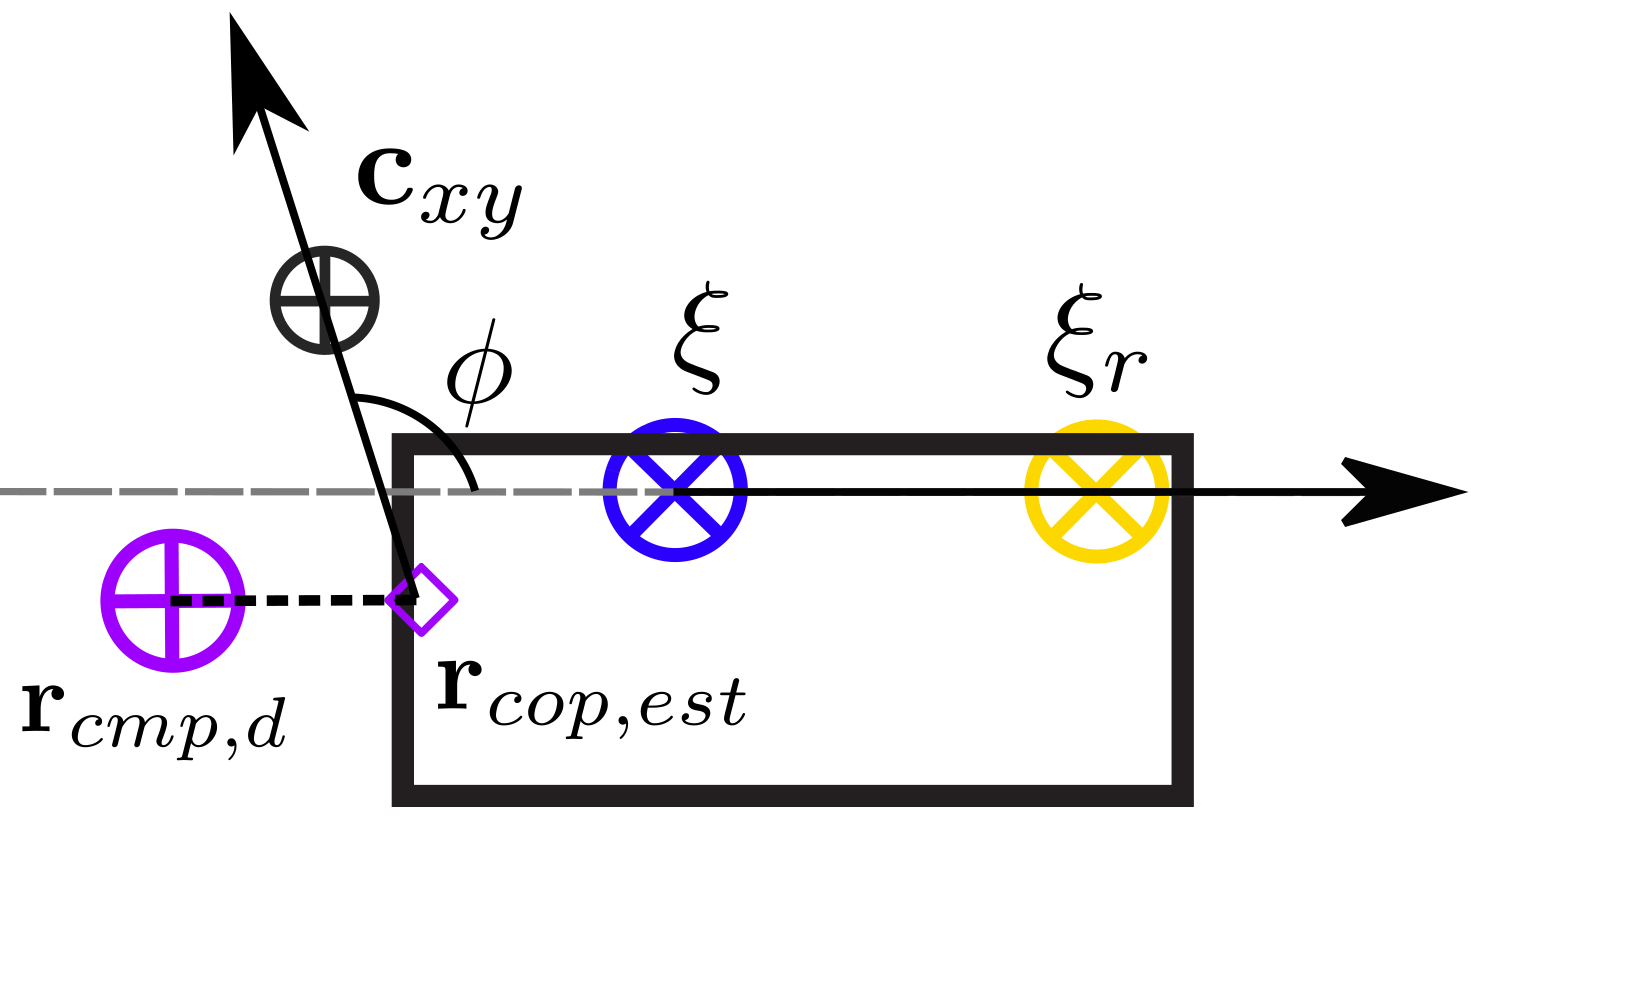
\includegraphics[width=.8\linewidth]{STYLESTUFF/ICPplanStartSSPhiViz.png}
   \caption{}
    \label{fig:phiViza}
  \end{subfigure}
  \begin{subfigure}{0.5\textwidth}
    \centering
  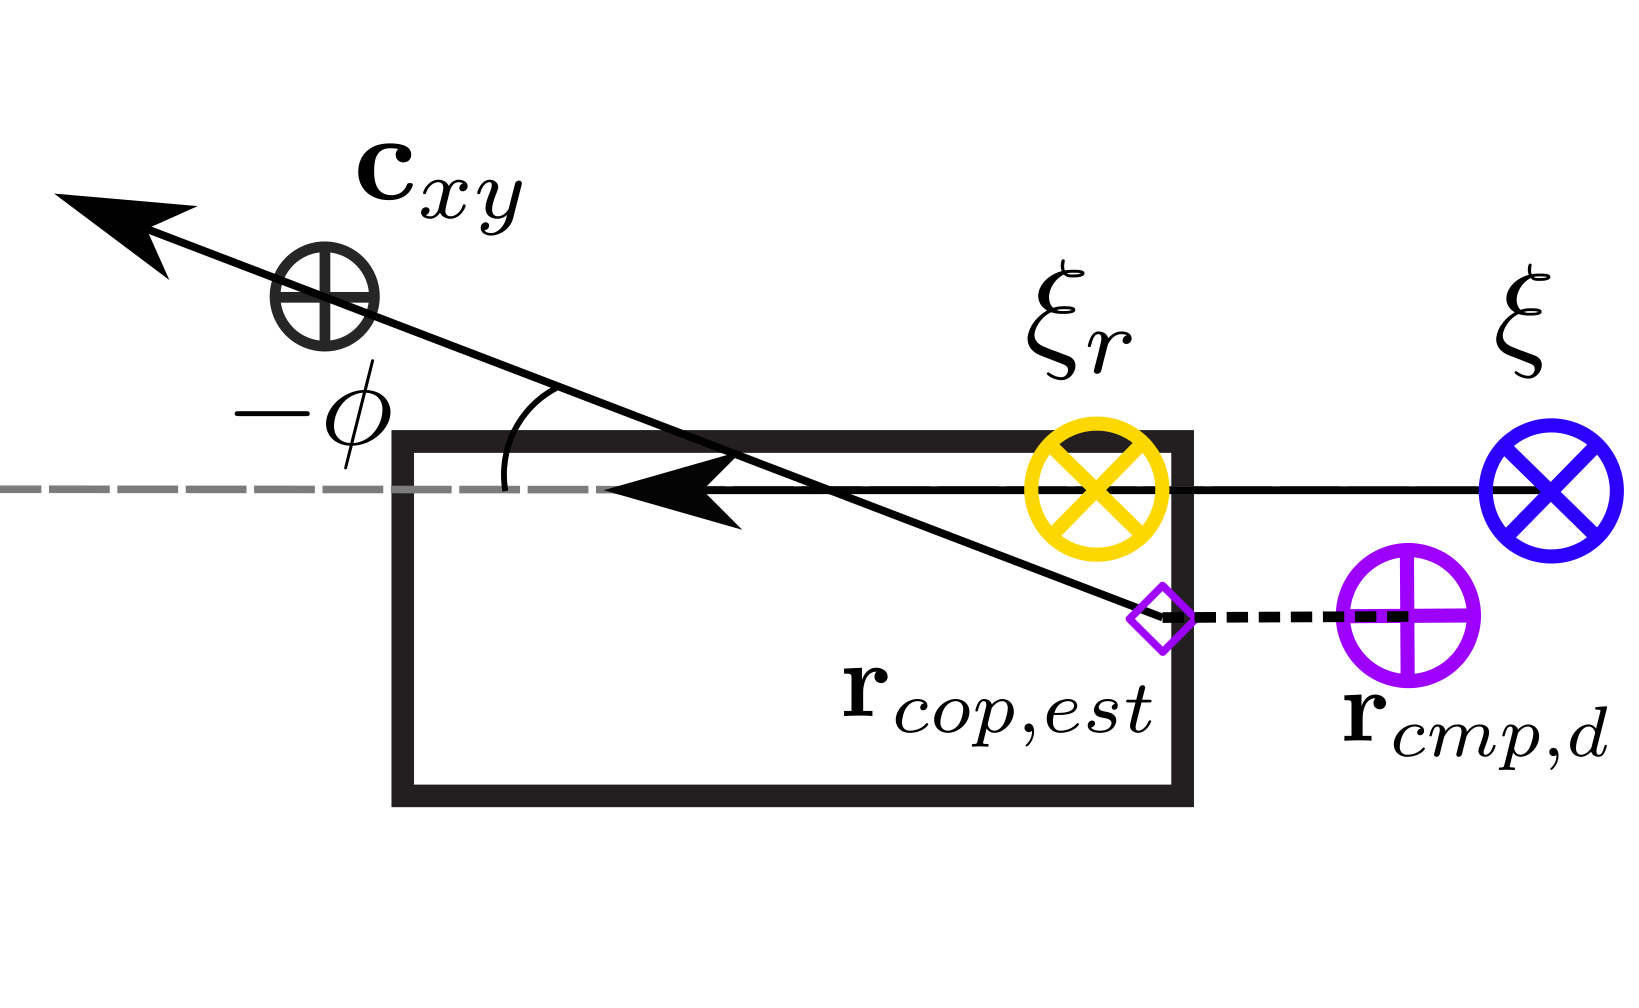
\includegraphics[width=.8\linewidth]{STYLESTUFF/ICPplanStartSSPhiVizNegError.png}
  \caption{}
   \label{fig:phiVizb}
  \end{subfigure}
  \begin{subfigure}{0.5\textwidth}
    \centering
  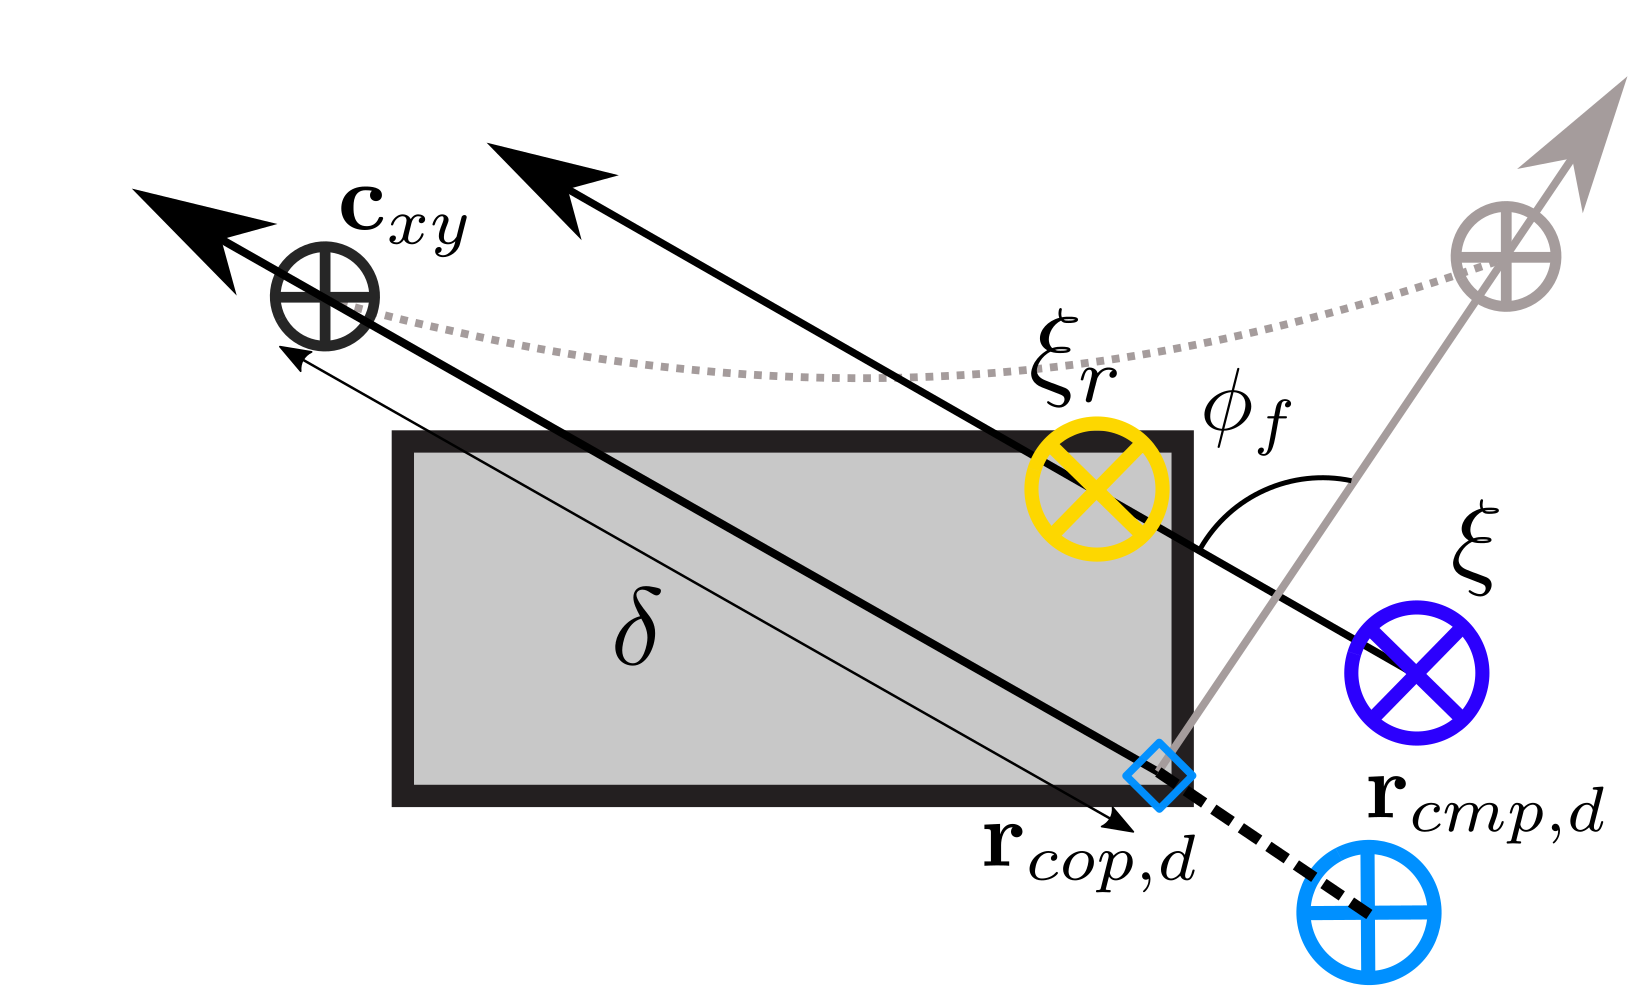
\includegraphics[width=.8\linewidth]{STYLESTUFF/ICPplanStartSSPhiViz0.png}
    \caption{}
     \label{fig:phiVizc}
  \end{subfigure}
  \begin{subfigure}{0.5\textwidth}
    \centering
  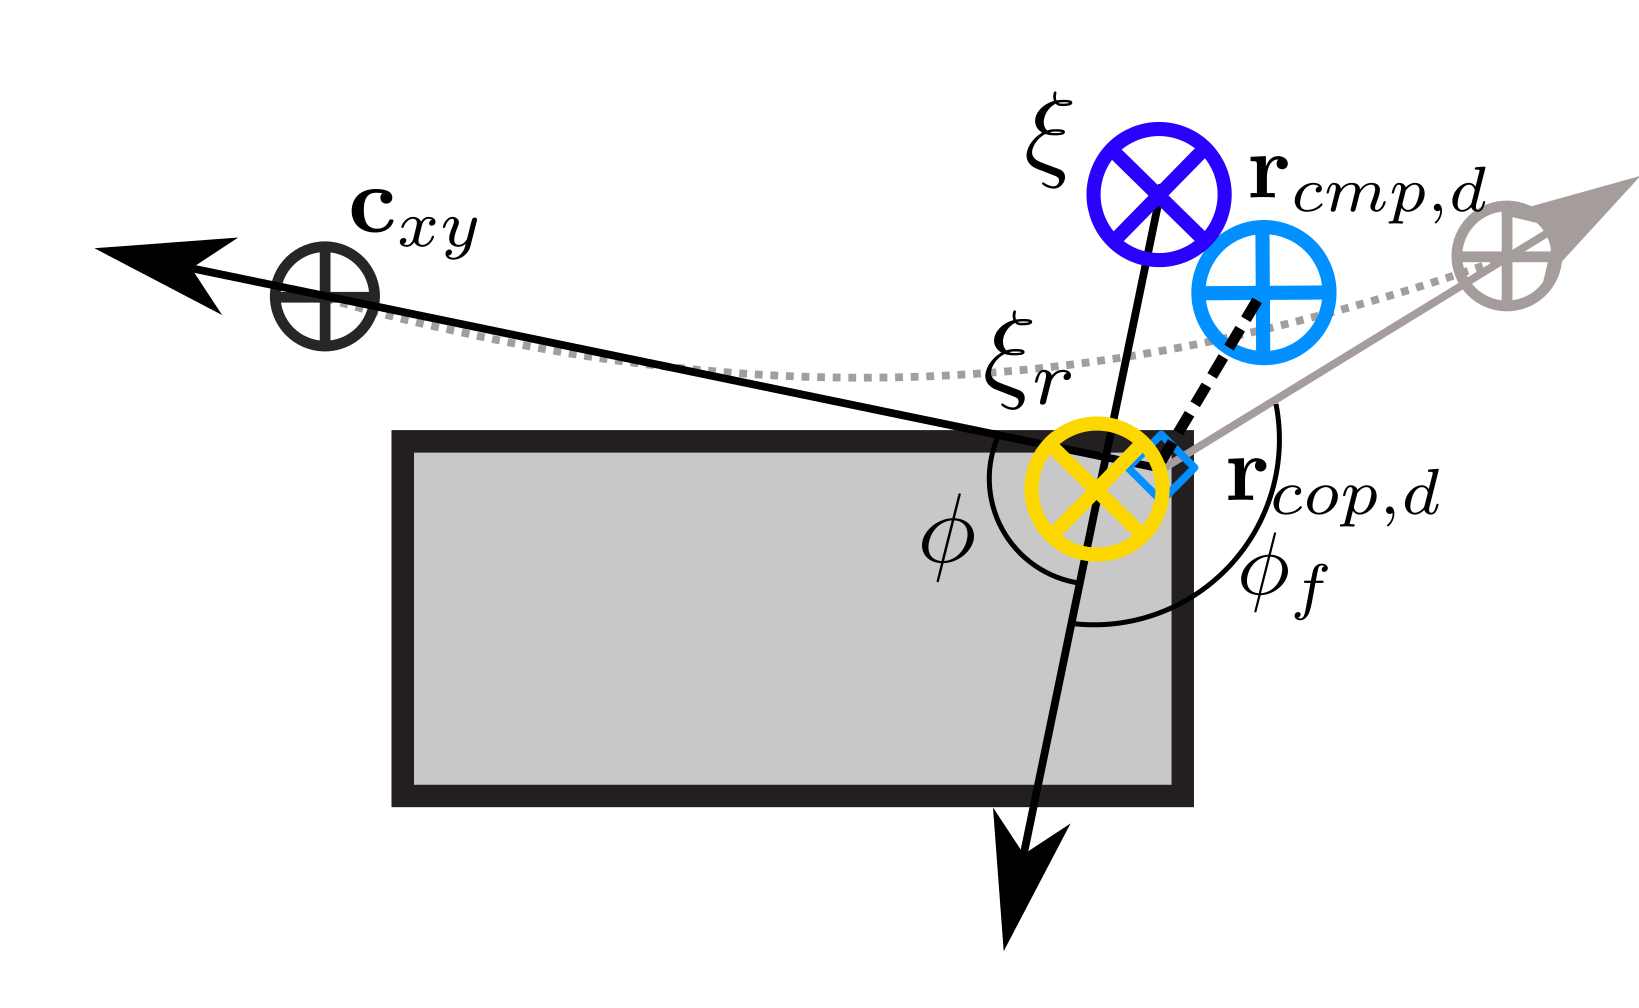
\includegraphics[width=.8\linewidth]{STYLESTUFF/ICPplanStartSSPhiViz90.png}
    \caption{}
     \label{fig:phiVizd}
  \end{subfigure}
    \begin{subfigure}{0.5\textwidth}
    \centering
  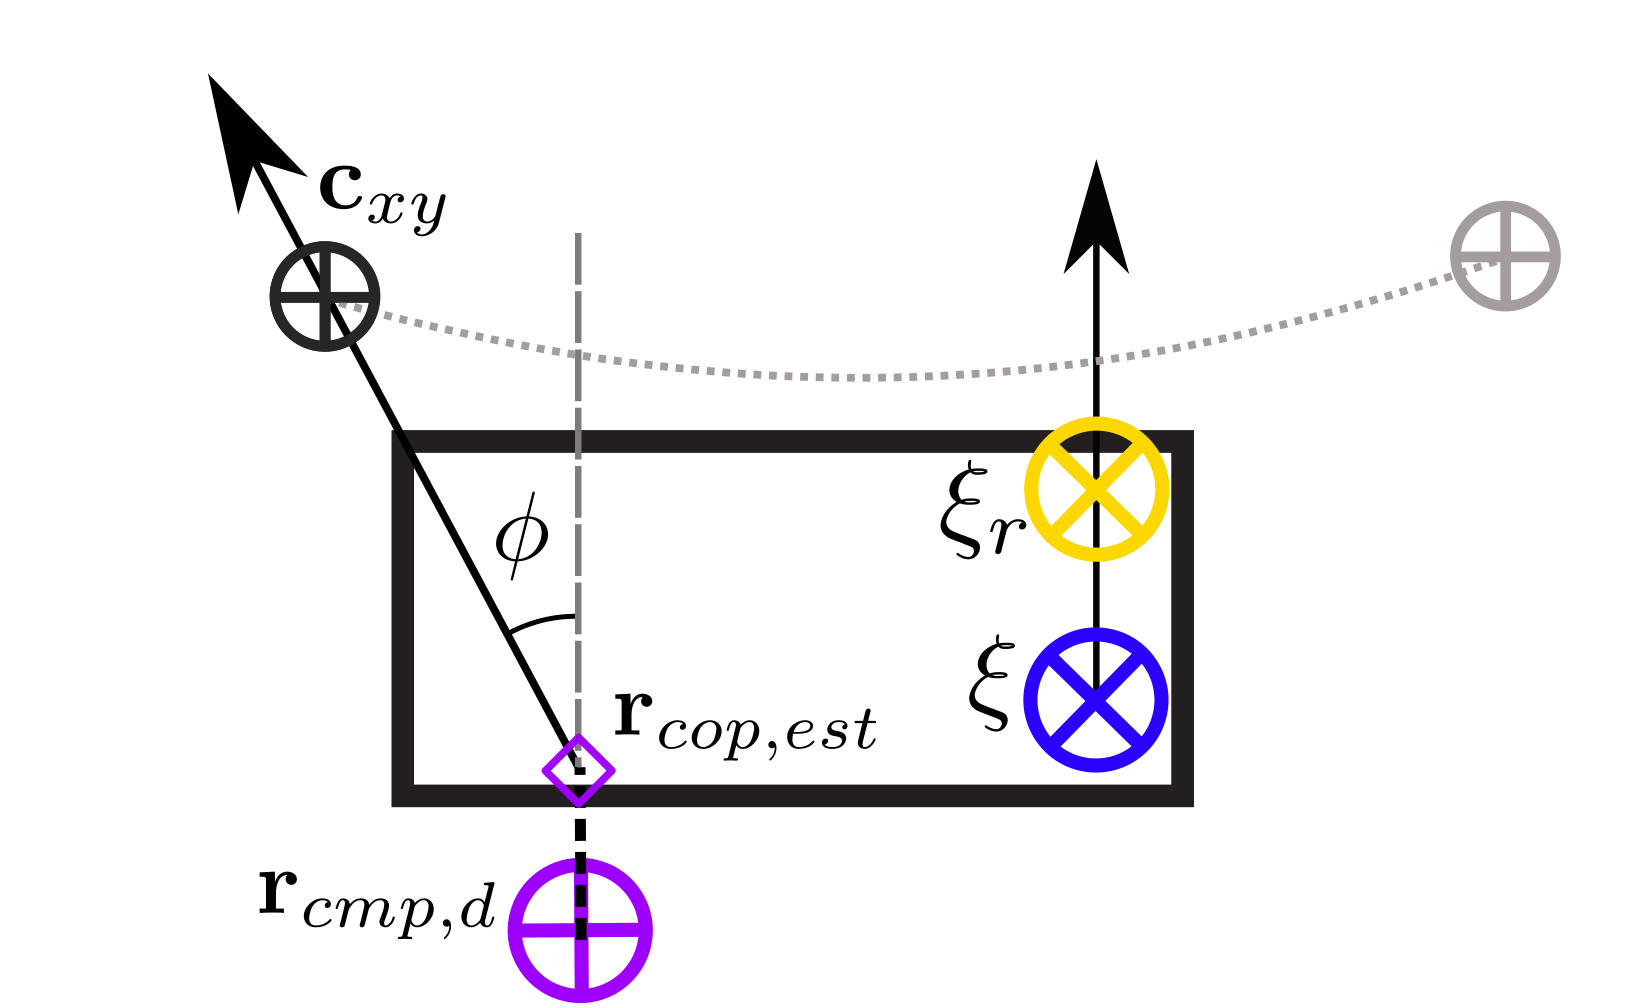
\includegraphics[width=.8\linewidth]{STYLESTUFF/ICPplanStartSSPhiVizLeftError.png}
    \caption{}
     \label{fig:phiVize}
  \end{subfigure}
  \begin{subfigure}{0.5\textwidth}
    \centering
  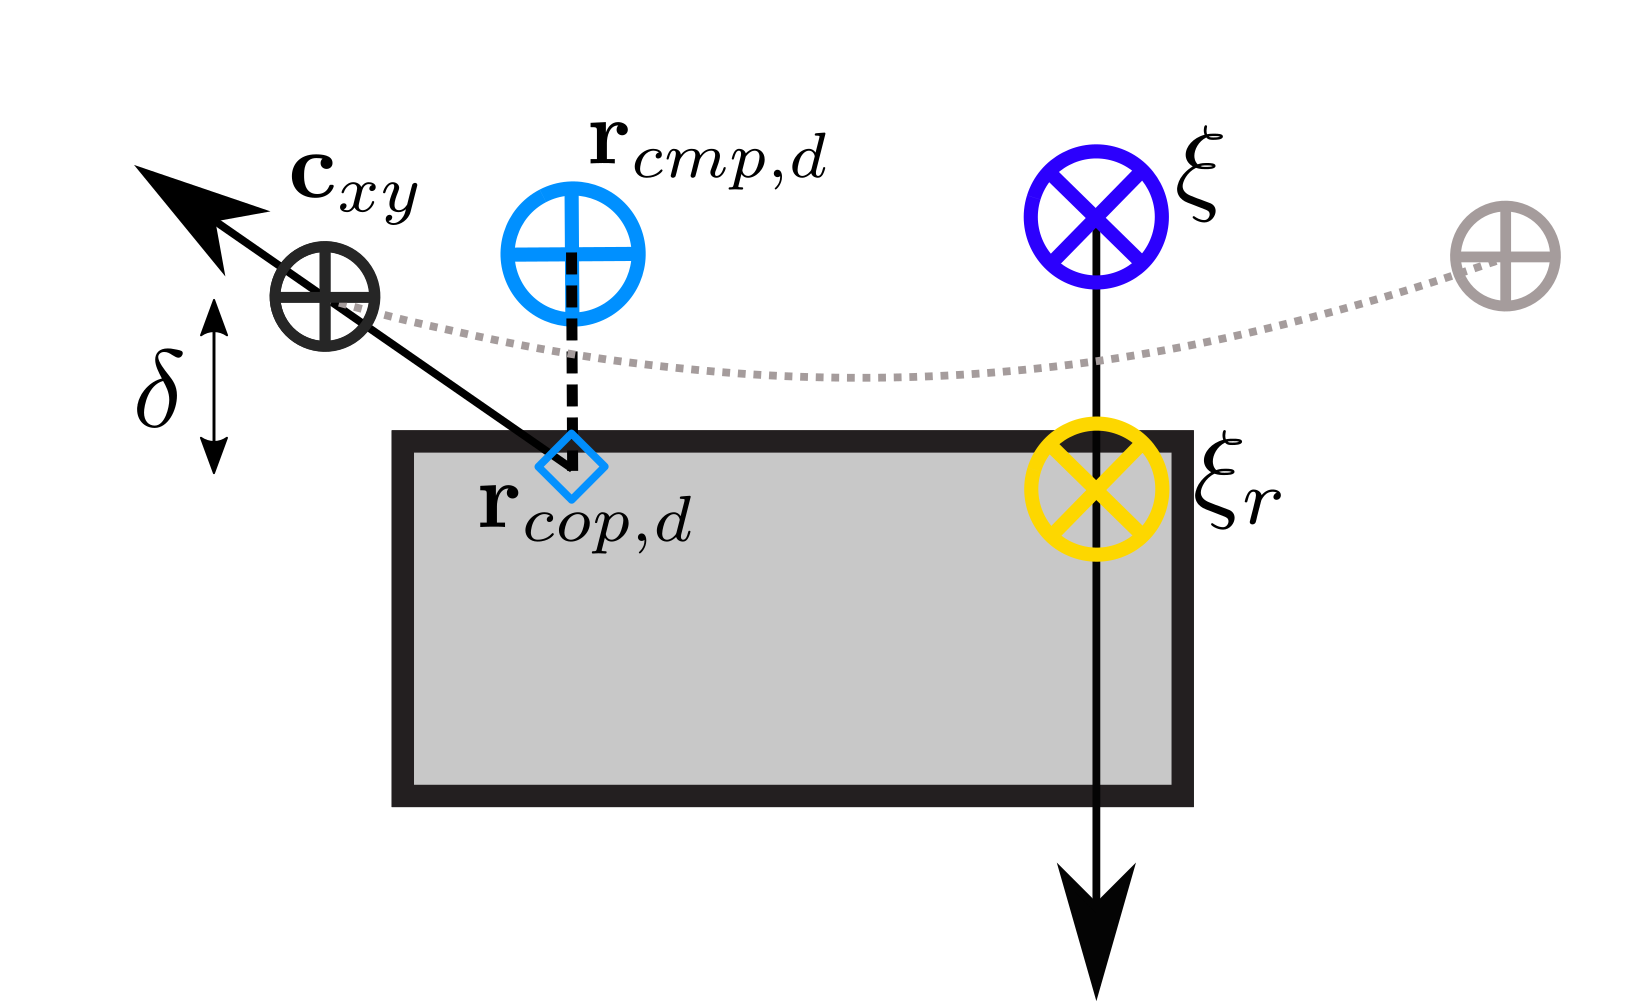
\includegraphics[width=.8\linewidth]{STYLESTUFF/ICPplanStartSSPhiVizRightError.png}
    \caption{}
     \label{fig:phiVizf}
  \end{subfigure}
  \caption{Vizualizations of the error alignment angle for the configuration at start of \ac{SS}, with \ac{ICP} errors: (a) negative in sagital plane, (b) positive in sagital plane, (c) where the error alignment angle is $0$ and (d) where the error alignment angle is orthogonal to the \ac{ICP} error. }
  \label{fig:phiViz}
\end{figure}


% Results
\clearpage
\section{Results}
\subsection{Standing}
Which cases?
\begin{itemize}
	\item Normal limit v.s. height control on normal limit
	\item Normal limit v.s. height control limit -> capture limits
	\item Normal limit high momentum weights v.s. height control on normal limit high momentum weights
\end{itemize}
\subsubsection{Simulation}
360 push.
\subsubsection{Hardware}
\begin{itemize}
	\item Increase $\ddzdmax$ until best found
	\item Front and side push
	\item Compare with normal config
	\item Compare with QP-based
	\item Compare with ang momentum
\end{itemize}
On what?
\begin{itemize}
	\item joint torques: ankle, knee, hip, back
	\item pose: angular momentum rate, angular momentum, body pose error, CoM
	\item reference points: CMP, CoP, ICP -> Integrated CoP effect and Angular effect > linear momentum
\end{itemize}

\subsubsection{Hardware Tests}
\subsection{Walking}
Focus on strategy.\\
Which cases? 
\begin{itemize}
	\item Normal limit v.s. height control on normal limit
	\item Normal limit v.s. height control limit -> capture limits? -> iterative push search.
\end{itemize}

On what?
\begin{itemize}
	\item ICP(t) v.s. ICPr(t) v.s. CoP(t) -> compare with assumptions
	\item Swing time and body pose.
\end{itemize}


% Discussion
\section{Discussion}
